\section{SHMAC}

SHMAC is a hardware prototype of a Single-ISA Heterogeneous MAny-core Com- puter
\cite{shmacsliedes, shmacwebpage}. It is an ongoing research project within the
Energy Efficient Computing Systems (EECS) research area at the Department of
Computer and Information Science at NTNU. The SHMAC project is driven by the
\textit{dark silicon effect}; as transistors become smaller, only parts of a
chip can be powered simulataneously. SHMAC implements two main strategies to
mitigate the dark silicon effect, heterogeneity and specialization.

\begin{figure}
    \centering
    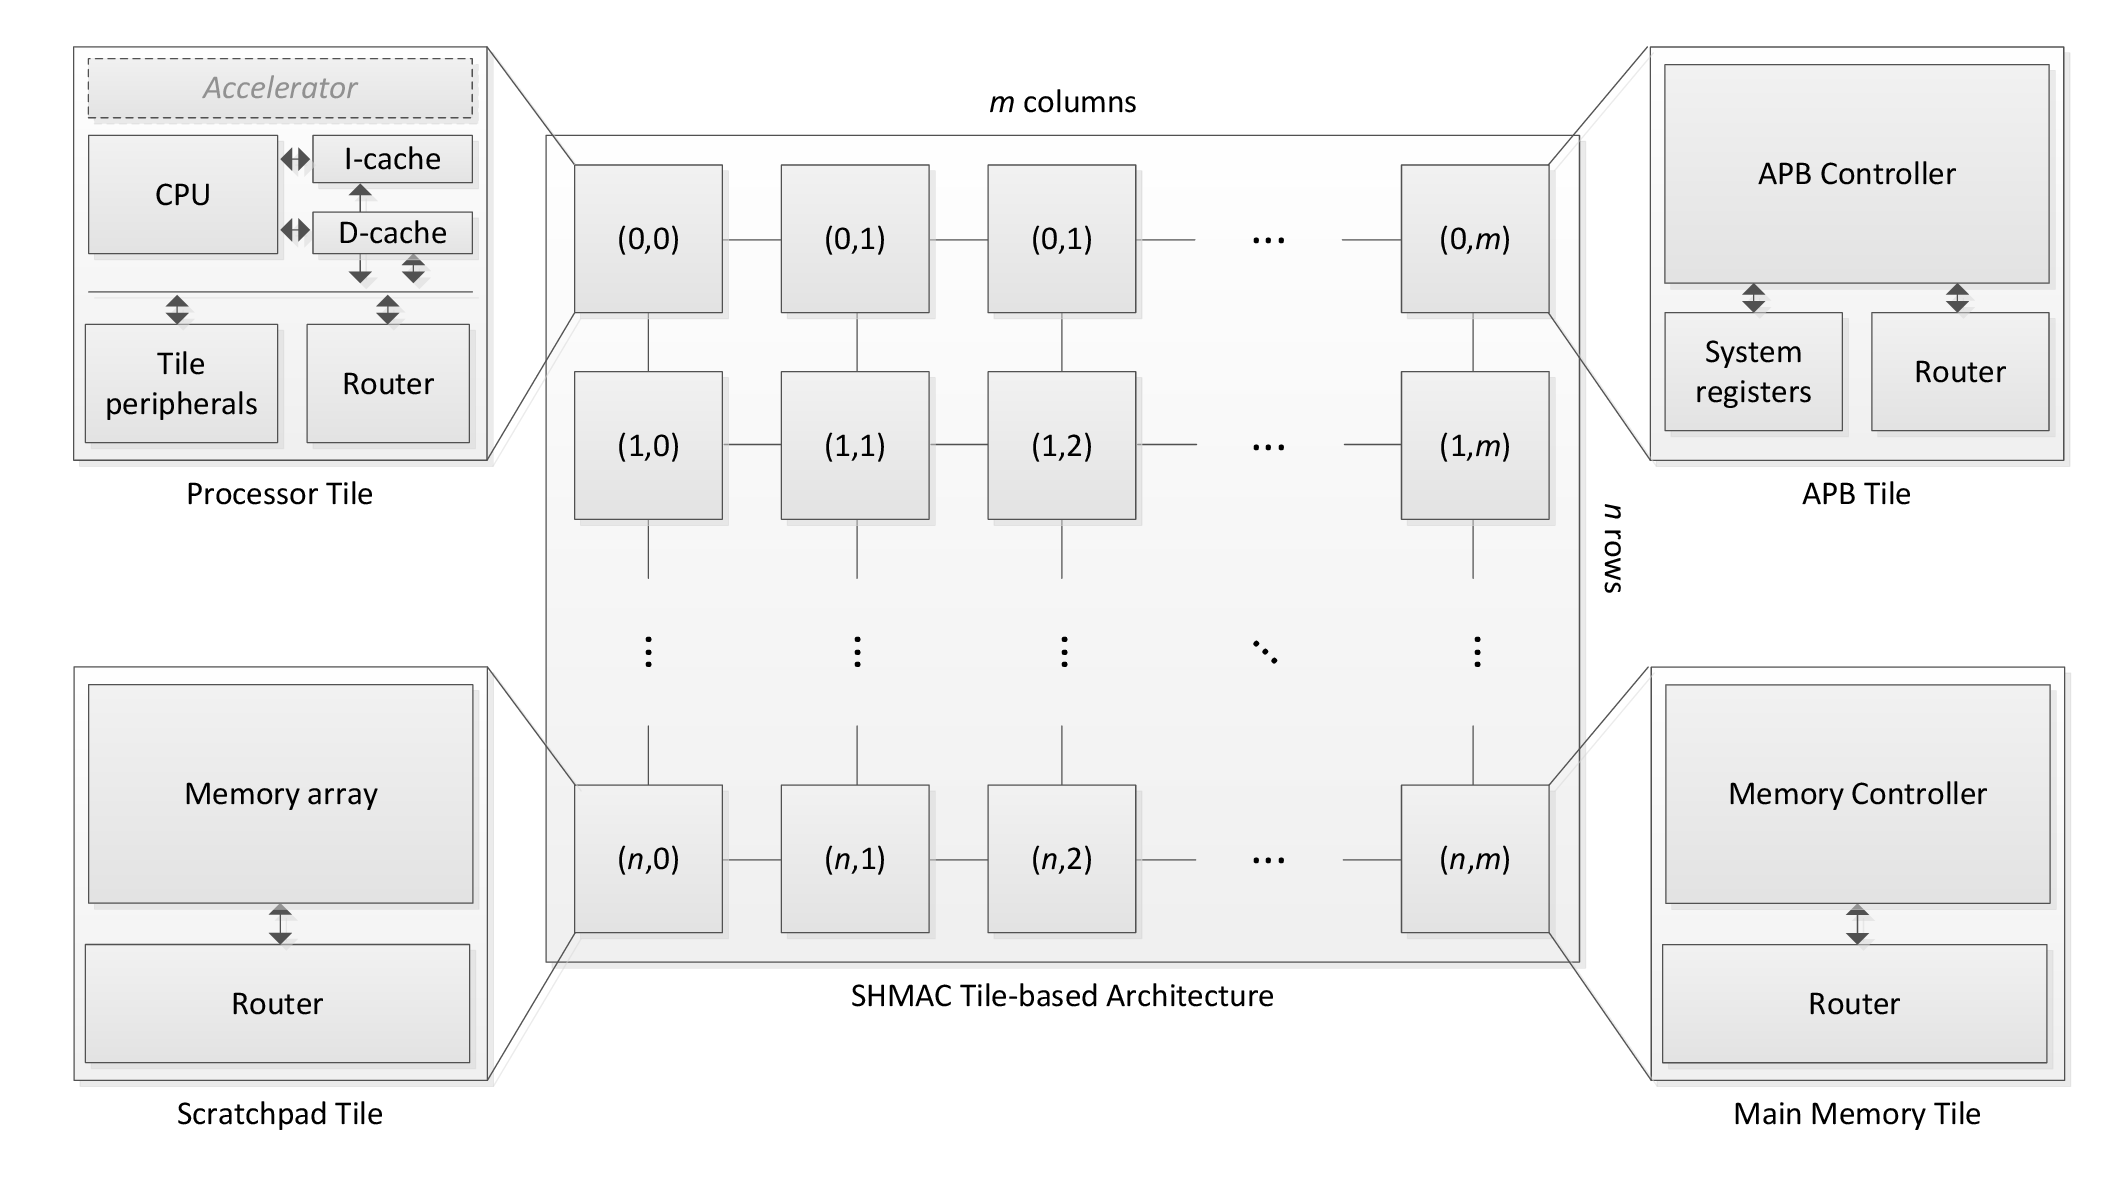
\includegraphics[width=1.0\textwidth]{figs/shmac-high-level2.png}
    \caption{}
    \label{fig:shmac}
\end{figure}

The SHMAC architecture is tile-based. Processing elements are laid out in a
rectangular grid with connections to their nearest neighbor, as depicted in
\autoref{fig:shmac}. A router protocol present in all SHMAC tiles handles
communication and data flow between tiles.  The great deal about SHMAC is that
different kinds of specialized tiles/accelerators can be composed as desired, to
form a computer tailored to the application.
